\chapter{Introducción}

Este trabajo se centra en dos temas: el tratamiento de imagen como una rama de conocimiento que está evolucionando en este momento y que se está empleando en el desarrollo de muchas investigaciones en diferentes campos y la docencia y lo importante que es que ésta sea accesible a todo el que esté interesado en aprender sobre un tema nuevo.\\

\section{Tratamiento de imagen}

La disciplina del tratamiento de imagen trata de la extracción de información de una o varias imágenes usando métodos matemáticos que tratan la imagen como una señal o matriz. Estos métodos pueden centrarse en mejorar la calidad de la imagen, añadir efectos o facilitar la búsqueda de información. El tratamiento digital de imagen usa ordenadores para aplicar estas transformaciones donde una imagen digital está compuesta de un número finito de elementos, cada uno con posición y valor particular (píxel).\\

Uno de los primeros ejemplos de tratamiento de imágenes digitales se dio en la década de los años 20 cuando se empezaron a enviar imágenes a través de un cable submarino de Londres a Nueva York. El sistema de transmisión de imágenes por cable de Bartlane usaba un telégrafo (Figura \ref{telegrafo}) para transmitir imágenes por el Atlántico. Inicialmente estas imágenes tenían 5 niveles de gris, pero fue ampliado a 15 niveles en 1929. Estas imágenes son consideradas las primeras imágenes digitales. La Figura \ref{1digital} muestra una imagen transmitida usando este sistema. Ya desde esta época se pudo ver que el principal problema que surgía con la imagen digital es la cantidad de espacio y capacidad computacional que requieren.\\

\begin{figure}[h]
\centering
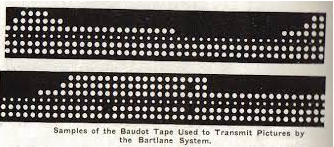
\includegraphics[width=0.8\textwidth]{imagenes/telegrafo}
\caption{Tira de Baudot.}
\label{telegrafo}
\end{figure}

\begin{figure}[h]
\centering
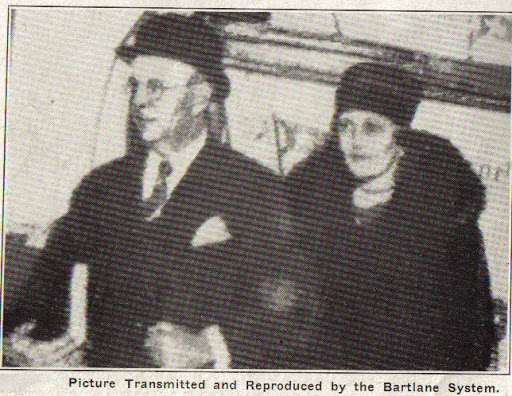
\includegraphics[width=0.8\textwidth]{imagenes/1digital}
\caption{Imagen transmitida usando el sistema de Bartlane.}
\label{1digital}
\end{figure}

Los avances en este campo en los primeros años dependían completamente del avance de los ordenadores y su capacidad tanto de almacenamiento como computacional.\\

Los primeros avances en el tratamiento digital de imágenes se dieron en los años 70 en el campo de la medicina y en astronomía. En medicina lo que impulsó esta necesidad para analizar imágenes digitales fué la invención del TAC (tomografía axial computarizada) que consiste en una serie de algoritmos que toman varias fotografías realizadas con rayos x para construir una imagen tridimensional. Se usan varias operaciones de tratamiento de imagen para mejorar el contraste de la imagen o pasar los diferentes niveles de gris a color para facilitar la interpretación.\\

Una de las razones principales que hacen que este campo sea tan complejo es la diferencia en cómo vemos imágenes nosotros y cómo las ``ve'' un ordenador. Nuestro cerebro analiza imágenes siempre en un contexto y con referencias para comparar, mientras que un ordenador recibe una serie de datos finitos en los que se ha perdido por el camino mucha información, por ejemplo si el objeto de la imagen es tridimensional, de dónde viene la imagen y el contexto de esa imagen. Esto hace que cosas que para la vista humana son obvias, para un ordenador sean operaciones muy complejas que requieran múltiples transformaciones y algoritmos para extraer ciertas características que se puedan contrastar con una base de datos.\\

El tratamiento de imagen se puede dividir en 3 procesos diferentes que se pueden dar secuencialmente en el análisis de una imagen o a la vez. Estos procesos son: pre-procesado, segmentación y análisis. La asignatura de TDI se centra sobre todo en métodos de pre-procesado y segmentación de imágenes.\\ 

\subsection{Aplicaciones}
El tratamiento digital de imagen tiene aplicaciones en una amplia variedad de campos desde medicina a diseño, pasando por astronomía y robótica.  Estos son algunos ejemplos de campos en los que se usan herramientas de tratamiento de imagen:
\begin{itemize}
\item \textbf{Medicina y biología}: El tratamiento de imágenes digital se usa para una gran cantidad de análisis. Un ejemplo serían las imágenes médicas que es el proceso de crear una representación visual de la estructura interior de un cuerpo antes de una intervención. También crea una representación visual de cómo funcionan varios órganos o tejidos. Esto se consigue gracias a varios avances en métodos como las tomografías computarizadas o las resonancias magnéticas.\\

También dentro del campo de la biología el tratamiento de imagen se está empleando para analizar imágenes sacadas de microscopio, por ejemplo para automatizar el cómputo de células en una imagen.\\

\item \textbf{Visión artificial y robótica}: Este campo consiste en intentar emular la visión humana usando el tratamiento de imagen. Su objetivo es reconocer objetos e información relevante de una forma similar a como lo hacemos los humanos. Se está aplicando sobre todo en el campo de la robótica, por ejemplo para casos como la conducción automática de los coches o robots.\\

\item \textbf{Restauración}: Otro campo en el que se usan las herramientas de tratamiento de imágenes es en la restauración de imágenes (figura \ref{restauracion} o videos dañados, ya sea por antigüedad o cualquier otra causa. \\

\begin{figure}[h]
\centering
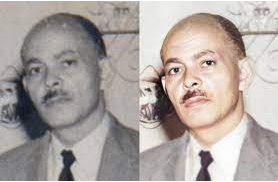
\includegraphics[width=0.8\textwidth]{imagenes/restauracion}
\caption{Imagen restaurada y coloreada usando tratamiento de imagen.}
\label{restauracion}
\end{figure}

\item \textbf{Geografía}: El tratamiento de imagen también se usa para crear mapas analizando imágenes de satélite y otros muchos análisis del terreno. Por ejemplo en agricultura Artizzu et al.\footnote{X. P. B. Artizzu, A. Ribeiro, A. Tellaeche, G.Pajares, C. F. Quintanilla (2009), Improving weed pressure assessment using digital images from an experience-based reasoning approach, Computers and Electronics in Agriculture, 65, pp. 176–185,
2009} diseñó un sistema que analiza imágenes del suelo y utiliza el color y la textura de la imagen para averiguar qué está plantado en esa zona.\\

\item \textbf{Seguridad}: Un tema por el que el tratamiento de imagen está recientemente en la noticias es su uso en seguridad, específicamente por la identificación facial en cámaras de seguridad. Este no es el único caso en el que se usa el tratamiento de imagen para seguridad, también se emplea en otras verificaciones biométricas, por ejemplo las huellas dactilares.\\

Otro ámbito de la seguridad en el que se usa el tratamiento de imagen es en la estenografía y la encriptación, por ejemplo para crear firmas digitales irremovibles en obras de arte o documentos.\\

\item \textbf{Transmisión y codificación}: Herramientas de tratamiento de imagen como el análisis de imágenes en frecuencia o  la reducción de niveles se usan amenudo para la codificación de imágenes y videos con el objetivo de que ocupen menos espacio y facilitar su transmisión.\\

\item \textbf{Diseño}: Por último mencionar el que seguramente sea el uso más común del tratamiento de imagen que es el diseño. Cualquier programa de uso común, como puede ser Photoshop, lo que tiene detrás de su interfaz son herramientas de tratamiento como filtros Gaussianos o filtros de detección de ejes.\\

\end{itemize}

\section{Educación accesible}

El tema principal de este proyecto es la educación como algo que debería ser gratuito y accesible al mayor número de personas posible

\section{La importancia de conocer las bases}

La razón por la que escogí 

